\section{Introduction}\label{sec:intro}

% batching is important
Transaction processing is a fundamental aspect of database functionality, and improving OLTP system performance has long been a key research goal in our community. It is well-known that the throughput of OLTP systems can be increased through \emph{batching}-based optimizations, whereby some component buffers a number of transactions or requests as they arrive and processes them as a group.

% batching for obvious reason: low level
Batching can improve system performance for several obvious reasons. First, it increases the efficiency of communication by packing messages~\cite{friedman1997packing,ding2015centiman}. Second, it amortizes the cost of system calls by condensing multiple requests into a single one, as in group commit~\cite{hagmann1987reimplementing, debrabant2013anti}. Third, it reduces the number of requests by discarding duplicate or stale ones, such as writes to the same record~\cite{faleiro2014lazy}. However, all of those are local optimizations based on low-level techniques.

% our proposal at a high level: batching at higher level for OCC 
We propose an OLTP system design that embraces batching as a core design principle at multiple stages of a transaction's execution. In particular, we explore the benefits of batching in optimistic concurrency control (OCC)~\cite{kung81tods} to reduce conflicts, and thus improve both system-wide and individual transaction performance. OCC is a popular concurrency control protocol~\cite{bernstein11cidr,bernstein11vldb, baker11cidr, patterson12vldb,peng10osdi,corbett12osdi, warp, bernstein2015optimizing} due to its low overhead in low-contention settings~\cite{adya97podc}. However, it wastes resources~\cite{agrawal1987concurrency} when conflicts are frequent. We show how batching reduces the number of conflicts and extends the applicability of OCC to higher-contention workloads.


Figure~\ref{fig:occ_arch} shows a distributed OCC-based transaction processing system with centralized validation. The system consists of three components: processors, storage nodes, and a single validator. External clients issue transactions to the system. On arrival into the system, each transaction is assigned to a processor and enters its \emph{read} phase. The processor sends read requests to the storage, executes the transaction, and performs ``writes'' to a local workspace. After it has processed the transaction, it sends information about the transaction's reads and writes to the validator. 

The transaction now enters the \emph{validation} phase. In OCC with \emph{backward validation}, the validator checks whether the transaction conflicts with any previously committed transactions, and makes a ``success'' or ``failure'' validation decision. One example of a conflict that would cause validation to fail is a \emph{stale read}. Suppose a transaction $t$ reads an object, and a second transaction $t'$ writes to the same object after $t$'s read. If $t'$ commits before $t$, $t$ has a conflict, since it should have read the update $t'$ made to the object but it did not. Thus $t$ must fail validation. 


If a transaction passes validation, the processor sends its writes to the storage; this is the \emph{write} phase. Otherwise, the processor aborts and restarts the transaction.

% why OCC for batching
The architecture of OCC with backward validation presents unique opportunities for batching because it contains multiple points of asynchronicity. 
% batching at processor
There are three obvious times and locations to apply batching. The first is the processor in the transactions' \emph{read} phase, where transaction requests can be batched before execution. There is recent work in the context of locking-based protocols that  batches transactions and serializes them before execution to reduce overheads~\cite{thomson2012calvin,faleiro2014rethinking,mu2014extracting}; these techniques could be adapted and applied in OCC as well.

% batching at validator
The second place we can batch is the validator, for transactions in the \emph{validation} phase. If the validator buffers the validation requests as they arrive, it has the flexibility to choose a validation order. This allows the validator to reduce the number of conflicts and aborts. Recall our previous example of a validation failure. A transaction $t$ reads an object, and a second transaction $t'$ writes to the same object after $t$'s read. If $t'$ arrives at the validator before $t$ and commits, $t$ must fail since it should have read the value written by $t'$ but it didn't. Instead, with batching, if transactions $t$ and $t'$ are both in the same batch waiting for validation, we can choose to serialize $t$ before $t'$. Thus, we avoid conflicts and both transactions can commit.

% batching at storage
Third, the system can perform batching at the storage level. This affects already-validated transactions in their \emph{write} phase as well as transactions that are still in their \emph{read} phase. The storage can buffer read and write requests into batches as they arrive. If a batch contains multiple read and write requests for the same object, the system can apply all the writes first, in the serialization order. Next, it can process the reads. Prioritizing writes over reads is always optimal in the sense that it reduces the number of aborts as much as possible. This is because OCC reads come from uncommitted transactions, while writes come from validated transactions that will commit soon. Thus if the storage has both a pending read and a pending write on the same object, but schedules the read before the write, the reading transaction will see a stale value and is guaranteed to fail the validation. 

% drawback of batching
Batching at these three levels in the system reduces aborts due to conflicts, and thus can increase throughput. However, it may also increase latency.

\begin{figure}[t]
 \centering
 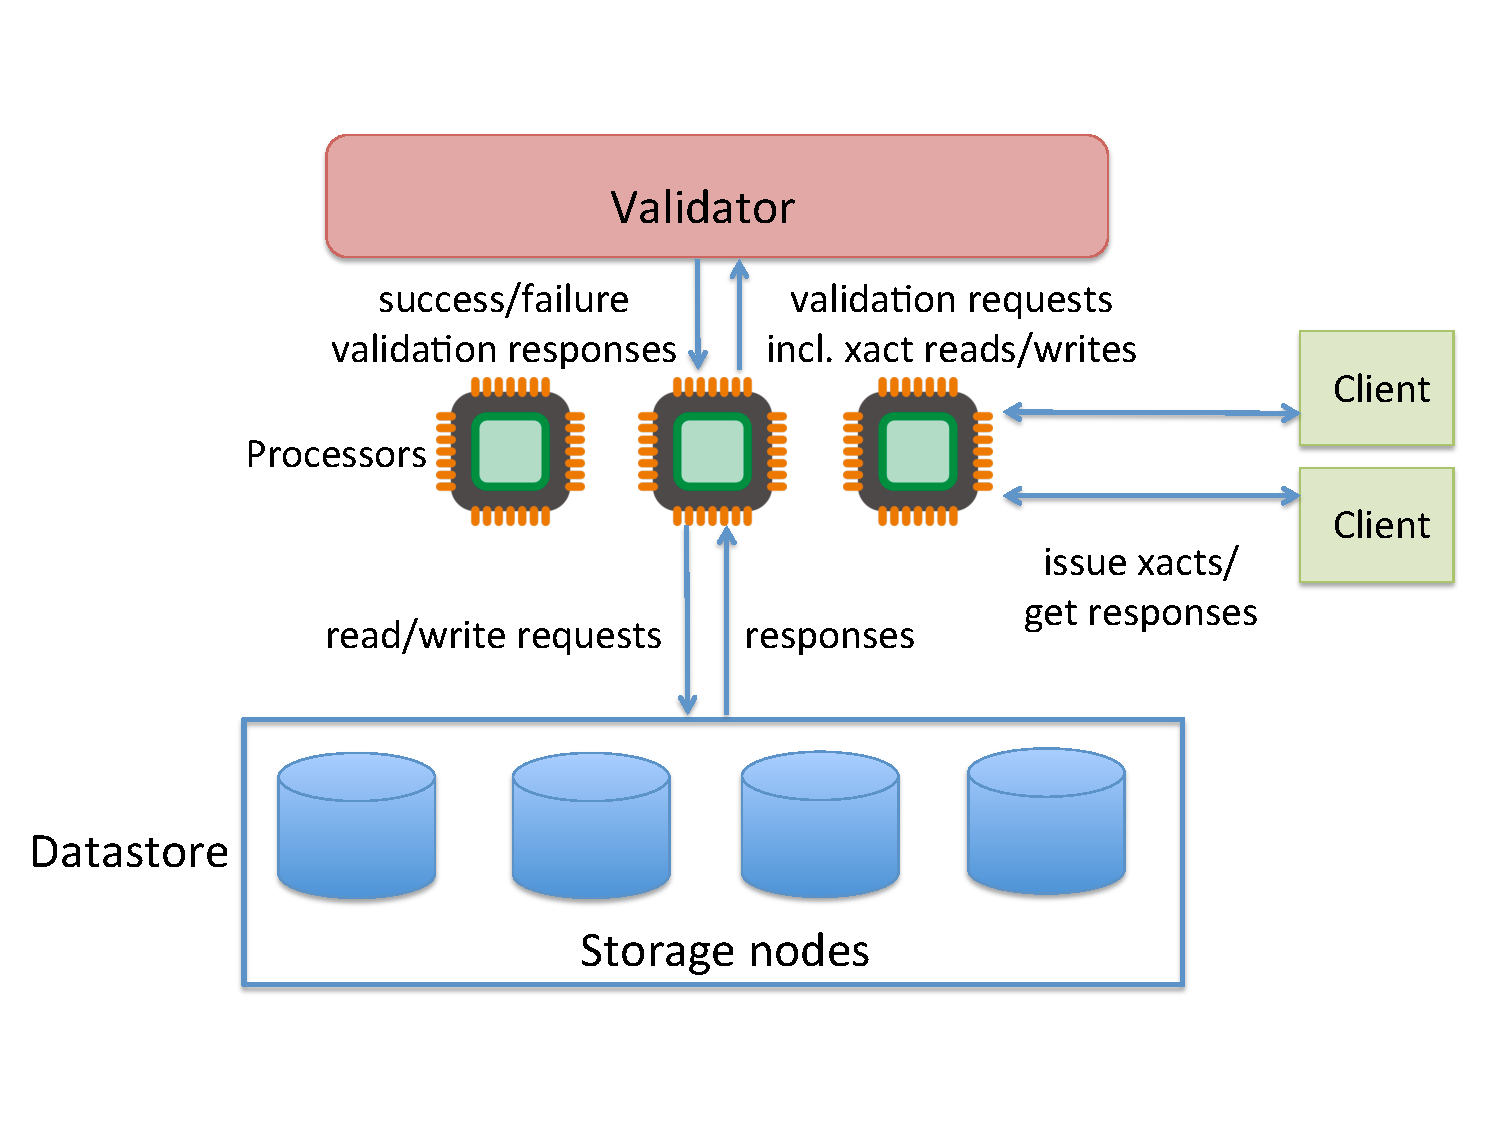
\includegraphics[width=0.9\columnwidth]{figures/OCCArchitecture.pdf}
 \vspace{-.5em}
 \caption{OCC System Architecture}
 \label{fig:occ_arch}
\end{figure}


% contribution
In this paper, we explore in-depth the benefits of transaction batching in OCC with backward validation. Since there is substantial existing work that applies directly to processor batching, we focus on storage and validator batching, which have received little research interest so far.

% contribution 1: system design
Our first contribution is an enhanced OCC system architecture that includes batching at the storage and the  validator levels. We analyze the reasons for conflicts and aborts at each stage of a transaction's life cycle, and develop techniques to reduce these aborts through batching.

% contribution 2: validator reordering algorithms
Our algorithmic focus is on validator batching, and more specifically on reordering within a batch at the validator. Optimal transaction reordering within a validator batch is NP-complete, as it can be formulated as the problem of finding a minimal feedback vertex set in a directed graph~\cite{karp1972reducibility}. Our second contribution consists of two classes of greedy algorithms. These algorithms produce feedback vertex sets that are not minimal but are a close approximation to the optimal solution, and they are fast enough to be used in practice. 

As mentioned before, the overhead of validator reordering increases transaction latency. Thus, even as validator reordering reduces the number of conflicts, it may hurt the end-to-end throughput of the system. Our two classes of greedy algorithms explore this trade-off. Additionally, we extend our algorithms to weighted versions that can incorporate features such as transaction priorities.

% contribution 3: experiment
Our third contribution is a detailed experimental study of the impacts of storage and validator batching in OCC.

% paper organization
The remainder of the paper is organized as follows. In Section~\ref{sec:background}  we review the fundamentals of OCC with backward validation. In Section~\ref{sec:overview} we discuss challenges, opportunities and techniques for storage and validator batching. In Section~\ref{sec:validator_reordering}, we introduce our algorithms for intra-batch transaction reordering at the validator. In Section~\ref{sec:experiments}, we present an extensive experimental study of batching throughout our system. We discuss related work in Section~\ref{sec:relwork} and conclude in Section~\ref{sec:conclusion}.

